\begin{problem}{Колесо в графе}{стандартный ввод}{стандартный вывод}{1 секунда}{256 мегабайт}

Коля по прозвищу <<Легенда>> придумал новый тип графов~--- \textit{колесо}. Колесом он называет граф, содержащий не менее 4 вершин, который можно изобразить на бумаге в виде <<колеса>>~ --- все вершины, кроме одной (которая является <<центром колеса>>) образуют цикл, и от каждой из них идёт по ребру к центру колеса. Других рёбер в графе нет.

Теперь Легенда ищет колеса во всех графах, которые он видит. Сегодня он смог раздобыть весьма интересный граф~--- неориентированный связный граф без петель и кратных ребер из $n$ вершин и $m$ ребер. Легенда хочет найти колесо в этом графе. Он считает, что в графе имеется колесо, если из графа можно убрать некоторые вершины и ребра таким образом, чтобы оставшийся граф стал этим самым колесом. 

Разумеется, Коля (Легенда) моментально нашел колесо (или понял, что нет никакого колеса), но он хочет проверить, сможете ли вы найти колесо? 

\InputFile
В первой строке заданы два целых числа $n$ и $m$ ($0 < n \leq 5000$, $0 \leq m \leq n \leq n (n-1) / 2$)~--- количество вершин и количество ребер в графе.

В следующих $m$ строках задаются ребра графа: в $i$-ой строке записаны два числа $u$ и $v$ ($0 < u, v \leq n$, $u \neq v$), означающие, что между вершинами $u$ и $v$ есть ребро.

\OutputFile
Если колес в графе нет, то выведите $-1$.

Иначе в первой строке выведите два числа: $k$ ($k \ge 4$)~--- количество вершин в найденном колесе и номер центра колеса, во второй строке~--- остальные $k-1$ вершин колеса в порядке обхода по циклу.

Если есть несколько колес, то выведите любое из них.

\Examples

\begin{example}
\exmpfile{example.01}{example.01.a}%
\end{example}
\begin{example}
    \exmpfile{example.02}{example.02.a}%
\exmpfile{example.03}{example.03.a}%
\end{example}

\Note
Иллюстрация к примеру 1: 

\begin{center}
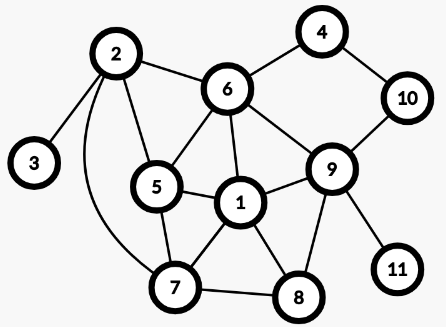
\includegraphics[scale=0.35]{image3.png}
\end{center}

В данном графе имеется два колеса: $\{1, 5, 6, 9, 8, 7\}$ и $\{5, 1, 7, 2, 6\}$.

\end{problem}

